\documentclass[a4paper,14pt]{extarticle}

% Шрифты, кодировки, символьные таблицы, переносы
\usepackage{cmap}
\usepackage[T2A]{fontenc}
\usepackage[utf8x]{inputenc}
\usepackage[english, russian]{babel}

% Пакеты американского математического сообщества
\usepackage{amssymb,amsfonts,amsmath,amsthm}  
% Сокращения
\usepackage{cancel}

\theoremstyle{definition}
\newtheorem{definition}{Определение}

% Красная строка
\usepackage{indentfirst}

% Ссылки в pdf
\usepackage[unicode, colorlinks, urlcolor=magenta, linkcolor=black]{hyperref}

% Таблицы
\usepackage{makecell,multirow} 

% Графика
\usepackage{graphicx}
\usepackage[usenames,dvipsnames]{color} 
\usepackage{float}
% \usepackage{subcaption}

% Геометрия страницы
\usepackage{geometry}
\geometry{left=2cm,right=2cm,top=2.5cm,bottom=2.5cm,bindingoffset=0cm,headheight=18pt}

% Колонтитулы
\usepackage{fancyhdr} 
% применим колонтитул к стилю страницы
\pagestyle{fancy} 
%очистим "шапку" страницы
\fancyhead{} 
%слева сверху на четных и справа на нечетных
\fancyhead[R]{Бугров А.В., Сарафанов Ф.Г.} 
%справа сверху на четных и слева на нечетных
\fancyhead[L]{Лекции по прикладной электродинамике} 
%очистим "подвал" страницы
\fancyfoot{} 
% номер страницы в нижнем колинтуле в центре
\fancyfoot[C]{\thepage} 

% Межстрочный отступ
\usepackage{setspace}
\linespread{1.15} % капельку увеличенный
\frenchspacing % <<французские>> пробелы

% Нумерация
\renewcommand{\labelenumii}{\theenumii)}
% В заголовках появляется точка, но при ссылке на них ее нет
\usepackage{misccorr}

% Содержание
\usepackage{tocloft}
\usepackage{secdot}
\sectiondot{subsection}

% Физика
\usepackage{physics}

% Новые команды
\newcommand{\Mean}[1]{\langle#1\rangle}
\newcommand{\Defi}{\underset{def}{=}}
\newcommand{\Inte}{\int\limits_{-\infty}^{\infty}} 

\addto\captionsrussian{%
	\renewcommand{\contentsname}{Оглавление}
	\renewcommand{\partname}{Часть}%
}
\def\thepart{\arabic{part}}
\usepackage{tocloft}
\renewcommand{\cftpartleader}{\cftdotfill{\cftdotsep}} % for parts
% \renewcommand{\cftchapleader}{\cftdotfill{\cftdotsep}} % for chapters
\renewcommand{\cftsecleader}{\cftdotfill{\cftdotsep}} % for chapters
% \newlength\mylen
\renewcommand\thepart{\arabic{part}.}
% \renewcommand\cftpartpresnum{Лекция~}
% \renewcommand\cftsecpresnum{Лекция~}
% \setlength{\cftsecnumwidth}{6em}
% \renewcommand{\cftsecpresnum}{Лекция\ }
% \renewcommand{\cftsecaftersnum}{.}
% \renewcommand{\cftsecaftersnumb}{\newline}
\renewcommand{\cftsecdotsep}{\cftdotsep}
\renewcommand{\kappa}{\varkappa}
\renewcommand{\phi}{\varphi}
\renewcommand{\epsilon}{\varepsilon}

% #1: math symbol
% #2: legend
\def\alegend#1#2{\overset{\underset{\scriptstyle\downarrow}{\scriptstyle\text{#2}}}{#1}}
\def\blegend#1#2{\underset{\underset{\scriptstyle\text{#2}}{\scriptstyle\uparrow}}{#1}}
\def\hp{\hat{p}}
\def\hx{\hat{x}}
\def\hH{\hat{H}}

% \usepackage[explicit]{titlesec}
% \titleformat{\section}{\normalfont\Large\bfseries}{}{0em}{Лекция\ \thesection.\ #1}
\usepackage{epigraph}


% \newcommand\praktika[1]{
% \stepcounter{section}
% \vspace{1.5em}
% \noindent\textbf{\Large{Занятие \arabic{section}.\hspace{.2em} #1}}
% % \newline 
% \vspace{-0.5em}
% \addcontentsline{toc}{section}{Занятие \arabic{section}.\hspace{.5em} #1}
% }

\usepackage{mathtools}
\mathtoolsset{showonlyrefs=true}


% https://tex.stackexchange.com/questions/8720/overbrace-underbrace-but-with-an-arrow-instead

\usepackage{xparse}% http://ctan.org/pkg/xparse

\NewDocumentCommand{\overarrow}{O{=} O{\uparrow} m}{%
  \overset{\makebox[0pt]{\begin{tabular}{@{}c@{}}$#3$\\[0pt]\ensuremath{#2}\end{tabular}}}{#1}
}
\NewDocumentCommand{\underarrow}{O{=} O{\downarrow} m}{%
  \underset{\makebox[0pt]{\begin{tabular}{@{}c@{}}\ensuremath{#2}\\[0pt]$#3$\end{tabular}}}{#1}
}

\newcommand\undernoteqty[2]{
	%
	\underarrow[
		\qty(\underbrace{#1})
	][\uparrow]{\substack{#2}}
	%
}

\newcommand{\pvec}[1]{\vec{#1}\mkern2mu\vphantom{#1}}
% Нормальный вектор для штрихов

\newcommand\undernote[2]{
	%
	\underarrow[
		#1
	][\uparrow]{\substack{#2}}
	%
}



% ##############################################################################
% ##############################################################################
\newcommand*\dotvec[1][1,1]{\crossproducttemp#1\relax}
\def\crossproducttemp#1,#2\relax{{\qty[\vec{#1}\times\vec{#2}\,]}}

\newcommand*\prodvec[1][1,1]{\crossproducttempa#1\relax}
\def\crossproducttempa#1,#2\relax{{\qty[{#1}\times{#2}\,]}}
% ##############################################################################
% ##############################################################################
\DeclareMathOperator{\Div}{div}
\DeclareMathOperator{\Rot}{rot}
\DeclareMathOperator{\Grad}{grad}
\begin{document}
%!TEX root = lections.tex
\begin{titlepage}
\thispagestyle{empty}

\begin{center}
	{\small\textsc{Нижегородский государственный университет имени Н.\,И. Лобачевского}}
	\vskip 3pt \hrule \vskip 5pt
	{\small\textsc{Радиофизический факультет}}

	\vfill

	\begin{spacing}{2}
	{\Huge \bf  Лекции по прикладной элекродинамике}\\%\vspace{1em}
	\end{spacing}
	\vspace{1em}
	{\Large Бугров А.В., Сарафанов Ф.Г.}\\[2em]
	{\large sfg180@yandex.ru}\\
	\vspace{1em}
\end{center}

\textbf{Disclaimer.} В данном документе нами набраны лекции по прикладной элекродинамике, прочитанные на 3 курсе радиофизического факультета ННГУ Владимиром Борисовичем Гильденбургом. Разрешено копирование и распространение данного документа с обязательным указанием первоисточника. 

\begin{center}
	\vfill
	28 февраля --- \today\\Нижний Новгород
\end{center}

\end{titlepage}
\newpage
\tableofcontents 
\newpage

\part{Электромагнитные волны в линиях передачи}
%!TEX root = ../lections.tex
 % Лекция от 06.02.2019 и начало лекции от 13.02, вплоть до "Волны в ЛП с идеальными ...."

\section{Волны в линиях передачи с идеально проводящими границами}
%!TEX root = ../lections.tex
\begin{figure}[H]
	\centering
	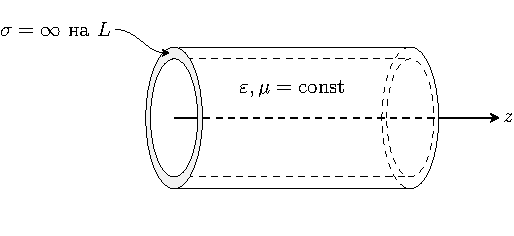
\includegraphics[scale=1.5]{img/lect2_ris1}
	\caption{Линия передачи}
	\label{fig:wavegain:1}
\end{figure}

\begin{figure}[H]
	\centering
	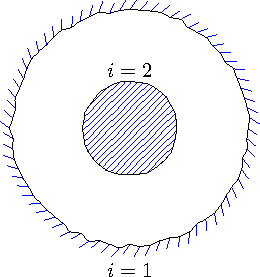
\includegraphics[scale=1.5]{img/lect2_ris2}
	\caption{Линия из разных проводников. Вид в разрезе}
	\label{fig:wavegain:2}
\end{figure}

\subsection{Математическая формулировка задачи отыскания волн в линиях передачи}

\begin{figure}[H]
	\centering
	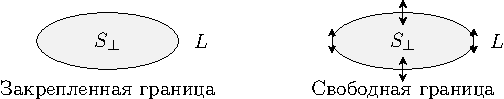
\includegraphics[scale=1.5]{img/lect2_ris3}
	\caption{Граничные условия Дирихле и Неймана в матфизике}
	\label{fig:wavegain:3}
\end{figure}

\begin{figure}[H]
	\centering
	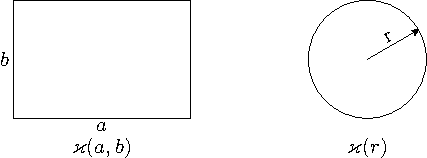
\includegraphics[scale=1.5]{img/lect2_ris4}
	\caption{Различная геометрия линии}
	\label{fig:wavegain:4}
\end{figure}

\begin{figure}[H]
	\centering
	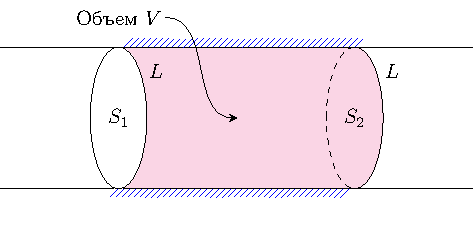
\includegraphics[scale=1.5]{img/lect2_ris5}
	\caption{Геометрия задачи}
	\label{fig:wavegain:5}
\end{figure}



\subsection{Дисперсионное уравнение}
Lorem ipsum dolor sit amet, consectetur adipisicing elit, sed do eiusmod
tempor incididunt ut labore et dolore magna aliqua. Ut enim ad minim veniam,
quis nostrud exercitation ullamco laboris nisi ut aliquip ex ea commodo
consequat. Duis aute irure dolor in reprehenderit in voluptate velit esse
cillum dolore eu fugiat nulla pariatur. Excepteur sint occaecat cupidatat non
proident, sunt in culpa qui officia deserunt mollit anim id est laborum.
\begin{figure}[H]
	\centering
	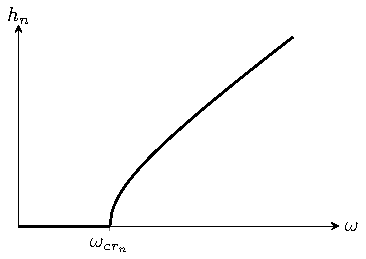
\includegraphics[scale=1.6]{img/lect2_ris6}
	\caption{Зависимость реальной части поперечного волнового числа от частоты}
	\label{fig:wavegain:5}
\end{figure} % Лекция от 13.02 начиная с этого заголовка

%!TEX root = ../lections.tex
\subsection{Моды в линиях передачи}
Любая мода в лии передачи характеризуется поперечным волновым числом, а поперечное волновое число определяет продольное.

Так же у нас есть дисперсионное соотношение:
\begin{equation}
	h = \pm \sqrt{\frac{\omega^2}{c^2} \varepsilon \mu -\kappa^2_n}
\end{equation}

Можем ввести критическую длину волны:
\begin{gather}
	\kappa^2 = {\frac{\omega}{c}}^2 {\epsilon \mu}\\
	\omega_{cr} = \frac{\kappa c}{\sqrt{\epsilon \mu}}\\
	\lambda = \frac{2 \pi c}{\omega_{cr}} = \frac{2 \pi}{\kappa \sqrt{\epsilon \mu}}
\end{gather}

Если задана $\omega_{cr} / \lambda_{cr}$ можем говорить, распространяется данная волна или нет.

Если волна бежит вправо, то $h > 0$; если бежит влево, то $h < 0$

При  $\omega > \omega_{cr}$- режим распространяющейся волны.

\begin{equation}
	Re{\vec{E}} , Re{\vec{H}} \sim \cos(\omega t - h z)
\end{equation}

\begin{figure}[H]
	\centering
	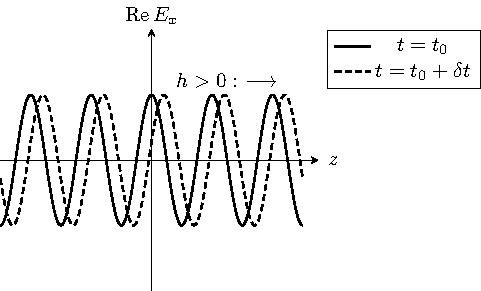
\includegraphics[scale=1.5]{img/lect3_ris1}
	\caption{Распространение волны ($h>0$)}
	\label{fig:lect3:1}
\end{figure}
При  $\omega < \omega_{cr}$- режим распространяющейся волны.

$h$ - мнимое.

\begin{equation}
	h = \pm i |h|
\end{equation}
\begin{equation}
	Re{E_x} \sim \cos(\omega t + \phi_0) \exp{\mp |h| z}
\end{equation}

Бегучести нет.

Зависимость экспонентальная
\begin{figure}[H]
	\centering
	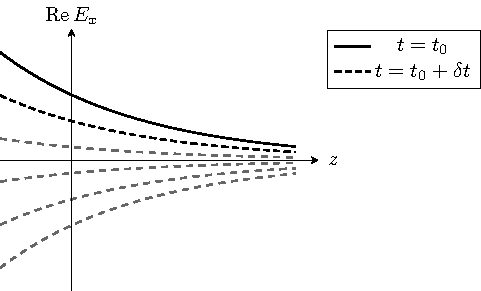
\includegraphics[scale=1.5]{img/lect3_ris2}
	\caption{Режим нераспространения ($h<0$)}
	\label{fig:lect3:2}
\end{figure}

\begin{figure}[H]
	\centering
	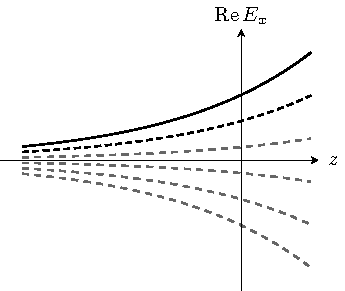
\includegraphics[scale=1.5]{img/lect3_ris3}
	\caption{Экспоненциальное нарастание амплитуды (при $h<0$)}
	\label{fig:lect3:3}
\end{figure}
Картинка зависит от способа создания волны, то есть у экспоненты " + или 		" - ". В зависимости от того, где источник можем сказать, куда бежит волна. То есть определить знак.

Источник может пораждать несколько мод, но не все, а какие-то конкретные.
\begin{figure}[H]
	\centering
	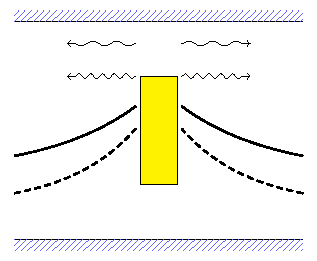
\includegraphics[scale=1.5]{img/lect3_ris4}
	\caption{Моды в линии передачи с источником}
	\label{fig:lect3:4}
\end{figure}
Изобразим числовую ось.
Пусть задана $\omega$, а то есть $k = \frac{\omega}{c} \sqrt{\epsilon \mu}$

Если $k < \kappa_1$ - все моды нераспространяющиеся.

Когда $k$ перейдёт через $\kappa_1$ появится низшая мода.

Когда перейдём через $\kappa_2$  появится ещё одна критическая частота.

!!Можно дополнить описание числовой прямой!!
\begin{figure}[H]
	\centering
	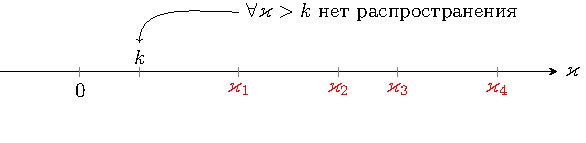
\includegraphics[scale=1.5]{img/lect3_ris5}
	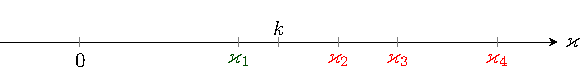
\includegraphics[scale=1.5]{img/lect3_ris6}
	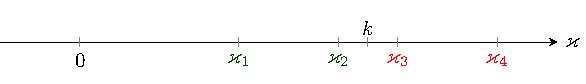
\includegraphics[scale=1.5]{img/lect3_ris7}
	% \label{fig:lect3:4}
\end{figure}

\subsection{Кинематические соотношения}
Определяют кинематические параметры волны.

\begin{enumerate}
	\item Временной период 

	\begin{equation}
		T = \frac{2 \pi}{\omega}
	\end{equation}

	\item Длина волны в волноводе (подразумевают линию передачи или трубу, когда говорят волновод)
	\begin{equation}
		\lambda_v = \frac{2 \pi}{h} = \frac{2 \pi}{\sqrt{k^2 - \kappa^2}} = \frac{2 \pi}{k} \frac{1}{\sqrt{1 - \frac{\kappa^2}{k^2}}} = \frac{\lambda_0}{\sqrt{1 - \frac{\omega_cr^2}{\omega}}} > \lambda_0
	\end{equation}

	Когда $\omega \rightarrow \omega_{cr}$	$\lambda_{v} \rightarrow \infty$

	$\lambda_0$ - длина волны в пространстве без волновoда в той же среде.

 	$\lambda_{v}$ - пространственный период.

 	\item Фазовая скорость - скорость перемещения плоскости постоянной фазы.

 	Поверхность постоянной фазы - это когда фаза константа.
 	\begin{equation}
 		faza = \omega t - h z + \phi_0
 	\end{equation}

 	При данном времени можно найти координату:
 	\begin{equation}
 		z = \frac{\omega t  + \phi_0}{ h }
 	\end{equation}

 	Координата будет перемещаться со скоростью:
 	\begin{equation}
 		v_f = \frac{\omega}{h}
 	\end{equation}
 	\begin{equation}
 		v_f = 
 		\frac{\omega}{\sqrt{k^2 - \kappa^2}} = 
 		\frac{\omega}{k} \frac{1}{\sqrt{1 - {\frac{k}{\kappa}^2}}} = \frac{\omega}{k} \frac{1}{\sqrt{1 - {\frac{\omega_{cr}}{\omega}^2}}} > v_f^{(0)}
	\end{equation}
	\begin{equation}
		v_f^{(0)} = \frac{c}{\varepsilon \mu} = \frac{\omega}{k}
	\end{equation}
 	Фазовая скорость может быть больше скорости света.

 	\item Групповая скорость - скорость перемещения квазимонохроматического волнового пакета. 

 	Волновой пакет - 

\begin{figure}[H]
	\centering
	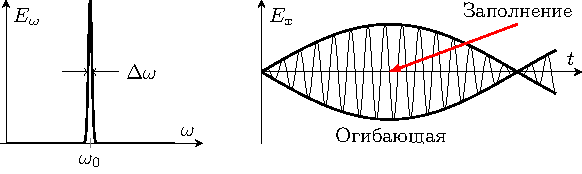
\includegraphics[scale=1.5]{img/lect3_ris8}
	\caption{Квазимонохроматический волновой пакет}
	\label{fig:lect3:8}
\end{figure}
	Сигнал характеризуется высокочастотным заполнением и огибающей.

\begin{figure}[H]
	\centering
	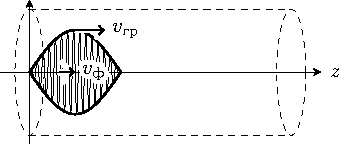
\includegraphics[scale=1.5]{img/lect3_ris9}
	\caption{Распространение волнового пакета}
	\label{fig:lect3:9}
\end{figure}
	По сути это радиоимпульс.

	Пакет движется со скоростью $ v_{gr} = \pdv{\omega}{k}\vert_{\omega = \omega_{0}} $ - это при малом или отсутствующем поглощении.(Это в пространстве, а не в линии передачи).

	При большом поглощении это понятие теряет смысл.

	По мере перемещения по волновду форма сигнала будет меняться.

	 $v_{gr} = \pdv{\omega}{h}\vert_{\omega = \omega_{0}} $ - формула для волновода. 

	 \begin{gather}
	 	k^2 = h^2 + \kappa^2\\
	 	%
	 	k = \frac{\omega}{c} \sqrt{ \varepsilon \mu}
	 \end{gather}

	Берём дифференциал от правой и левой части.$\kappa$  не зависит от частоты.
	\begin{gather}
		2k dk = 2h dh\\
		\pdv{\omega}{h} = \frac{c}{\sqrt{\varepsilon \mu}} \frac{h}{k}\\
		h = + \sqrt{\frac{\omega^2}{c^2} \varepsilon \mu -\kappa^2_n}\\
		\pdv{\omega}{h} = \frac{c}{\sqrt{\varepsilon \mu}} \frac{c}{\omega \sqrt{\varepsilon \mu}} \sqrt{\frac{\omega^2}{c^2} \varepsilon \mu -\kappa^2_n} = \frac{{v_f^{(0)}}^2}{v_f}
 	\end{gather}

 	\begin{gather}
 		v_{f} = \frac{\omega}{h}\\
 		v_{f}^{(0)} = \frac{c}{\omega \sqrt{\varepsilon \mu}}\\
 		%
 		v_{f} v_{gr} = {v_f^{(0)}}^2
 	\end{gather}
 	\begin{equation}
 		v_{gr} = v_{f}^{(0)} \sqrt{1 - {\frac{\omega_{cr}}{\omega}^2}}
 	\end{equation}

	Всё это справедливо для сред без временной дисперсии.
	\begin{equation}
		\varepsilon\ne f(\omega), \mu \ne f(\omega)
	\end{equation}

	!! есть ещё комментарии про дисперсию!!

	$v_{gr} < c$ - она несёт информацию.
\end{enumerate}
\begin{figure}[H]
	\centering
	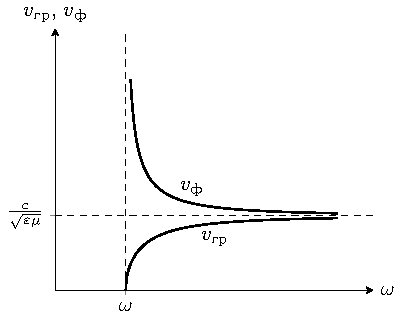
\includegraphics[scale=1.5]{img/lect3_ris10}
	\caption{Распространение волнового пакета}
	\label{fig:lect3:10}
\end{figure}

\subsection{Потоки энергии в линии передачи}
Когда идёт волна в линии передачи она переносит энергию.

Поток энергии характеризуется вектором Пойнтинга.

\begin{equation}
	\vec{S} = \frac{c}{4 \pi} [ Re{\vec{E}}, Re{\vec{H}}]
\end{equation}

Необходимо, чтобы уравнения были линейными
\begin{equation}
	Re{\vec{E}} Re{\vec{H}} \neq Re{(\vec{E} \vec{H})}
\end{equation}

Важная величина - среднее по времени.

Пусть есть
\begin{equation}
	A = A_0 \exp{i \omega t}
\end{equation}
\begin{equation}
	B = B_0 \exp{i \omega t}
\end{equation}
\begin{equation}
	\overline{Re{A}Re{B}} = \frac{1}{T} \int{Re{A}Re{B}}dt = \frac{1}{2} Re{A B*}
\end{equation}
где $\overline{A}$ - усреднение по времени, $B*$ - комплексно - сопряженное значение.
\begin{equation}
	\overline{\vec{S}} = \overline{\frac{4 \pi} [Re{\vec{E}}, Re{\vec{H}}]} = \frac{c}{8 \pi} Re[\vec{E}, \vec{H*}]
\end{equation}

 $\Sigma$ -  поперечное сечение линии передачи. 
Средний по времени поток:
\begin{equation}
	\Pi = \iint_{\Sigma} \overline{S_z} ds
\end{equation}
Поток - количество энергии, которое переносится через поперечное сечение за одну секунду.
$\overline{S_z}$ - проекция вектора Пойнтинга на ось z.
Вклад дают поперечные компоненты (в проекции на ось z).
\begin{equation}
	\overline{S_z} = \frac{c}{8 \pi} Re([\vec{E_\perp}, \vec{H*_\perp}], \vec{z_0})
\end{equation}
Можно переписать, если использовать соотношение:

\begin{equation}
	\vec{E_\perp} = \vartheta_{v \perp} [\vec{H_\perp}, \vec{z_0}]
\end{equation}
это в бегучей волне.

Подставив:
\begin{equation}
	\Pi = \frac{c}{8 \pi} Re{\vartheta_{v \perp}} \iint_{\Sigma} |\vec{H_\perp}|^2 ds
\end{equation}
или по-другому:
\begin{equation}
	\Pi = \frac{c}{8 \pi} 
		Re{\frac{1}{\vartheta_{v \perp})}} \iint_{\Sigma} |\vec{E_\perp}|^2 ds
\end{equation}
$\Pi$ ещё называют средней мощностью волны.
\begin{equation}
	\vartheta_{v \perp} = \sqrt{\frac{\mu}{\varepsilon}} {\frac{k}{h}}^{\pm 1}
\end{equation}
+ для ТЕ, - для ТМ.
$\omega < \omega_{kr}$- уравнение имеет только мнимые решения.
$h_n = 0$; 

Тогда $\vartheta_{v \perp}$  - мнимое, $Re$ часть равна нулю и поток энергии равен нулю.

$\omega > \omega_{kr}$ - мода имеет действительное h, волна распространяющаяся.
 $\vartheta_{v \perp}$- действительное, его реальная часть не равна нулю,поток энергии не равен нулю.
А что если в линии передачи несколько типов волн:

Пусть есть - $N$ мод.
\begin{equation}
	\Pi = \Sigma^{N}_{i = 1} \Pi_i
\end{equation}

Полный поток - сумма порциальных потоков.
Но здесь речь идёт о среднем.
 % Лекция от 20.02

\newpage
%!TEX root = ../lections.tex
\subsection{Главные (TEM) волны в линиях передачи с идеальными границами}

У TEM-волн поперечное волновое число $\varkappa=0$:
\begin{equation}
	\varkappa=0 \Rightarrow h=k= \frac{\omega}{c}\sqrt{\varepsilon \mu}
\end{equation}
Поля таких волн выражаются следующим образом через функцию $\varphi$:
\begin{gather}
	\label{eperp}
	\vec{E}_\perp=-\frac{1}{\sqrt{\varepsilon \mu}}\nabla_\perp \varphi\\
	\vec{E}_\perp=-\frac{1}{\mu}\qty[\nabla_\perp \varphi,\vec{z}_0]
\end{gather}

При этом выполняются \textbf{граничные условия}: на каждом из проводников (допустим, есть набор проводников, вдоль которых распространяется волна)
\begin{equation}
	\varphi|_{l_i}=C_i,
\end{equation}
причем константа не обязана быть одна для всех проводников.

\begin{figure}[H]
	\centering
	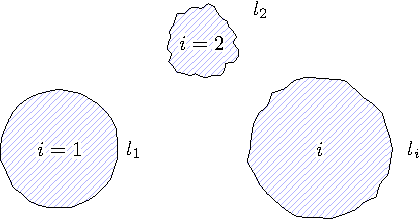
\includegraphics[scale=1.5]{img/lect4_ris1}
	\caption{Набор проводников в задаче}
	\label{fig:lect4:1}
\end{figure}

\subsubsection{Внутренняя задача}
\begin{figure}[H]
	\centering
	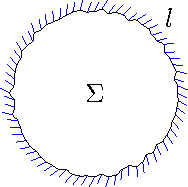
\includegraphics[scale=1.5]{img/lect4_ris2}
	\caption{Случай одного проводника}
	\label{fig:lect4:2}
\end{figure}
Пусть у нас есть только один проводник, в котором есть цилиндрическая полость (рис. \ref{fig:lect4:2}). Рассмотрим внутреннюю задачу, т.е. распространение волны внутри цилиндрической полости. Оказывается, для граничного условия $\varphi_\perp|_l=C_1$ существует только тривиальное решение $\varphi_\perp=C_1$. В матфизике это доказывается. Начало доказательства такое:

\begin{equation}
	\Delta \varphi=\Div\qty(\varphi\nabla \varphi)=0 \quad \bigg| \iint\limits_\Sigma
\end{equation}
Это такая задача, которую проще доказать самому. Попробуйте это сделать сами.

\subsubsection{Внешняя задача}
Зададимся вопросом о решении той же задачи:
\begin{equation}
	\Delta_\perp \varphi=0, \quad \varphi|_l=\mathrm{const}
\end{equation}
Только теперь будем рассматривать её в области вне проводника, т.н. внешняя задача.

Для начала рассмотрим задачу попроще, поле нити (рис. \ref{fig:lect4:3}). Решение её известно:
\begin{equation}
 	\Delta_\perp \varphi=0 
 		\quad \Rightarrow \quad
 	\varphi \sim \ln r
\end{equation} 

Характер убывания полей здесь $E_r\sim \frac{1}{r}$, а для магнитного поля в силу импедансного соотношения $\frac{E_r}{H_\phi}=\eta_{\perp\text{в}}=1$ $H_\varphi\sim\frac{1}{r}$:
\begin{equation}
	E_r=H_\phi\sim\frac{1}{r}
\end{equation}
\begin{figure}[h!]
	\centering
	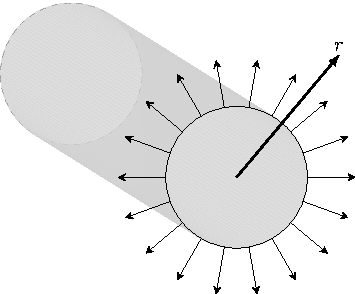
\includegraphics[scale=1.5]{img/lect4_ris3}
	\caption{Поле бесконечной проводящей нити}
	\label{fig:lect4:3}
\end{figure}

Посмотрим на поведение полей при $r\to\infty$. Говорят, нужно поставить граничные условия (или закон убывания) на бесконечности. Чем плох закон $\frac{1}{r}$?

Посчитаем средний по времени поток энергии через поперечное сечение, в котором распространяется волна. Сечение бесконечно, за исключением конечной площади проводника.

Сначала вычислим вектор Пойнтинга (средний по времени и в проекции на $z$):
\begin{equation}
	\overline{S}_z=\frac{c}{8 \pi}\mathrm{Re}\qty(E_r\cdot H_\phi^*)\sim\frac{1}{r^2}
\end{equation}
\begin{equation}
	\Pi=\iint\limits_\Sigma \overline{S}_z ds \sim
	\iint\limits_\Sigma \frac{1}{r^2} (2\pi r \dd{r})
	\sim \int\limits_a^\infty = \ln\frac{\infty}{a}=\infty
\end{equation}
Интеграл расходится на бесконечности. Говорят, что расходимость носит логарифмический характер. Получили бесконечную мощность волны: такую волну невозможно создать реальным источником --- волна не удовлетворяет критерию энергетической реализуемости.

Можно сделать важный вывод: \textbf{вдоль одиночного проводника TEM-волна с конечной энергией распространятся не может}. А может,если проводников больше. Например, в линии из двух проводников (рис. \ref{fig:lect4:4}) TEM-волна уже возможна.

\begin{figure}[H]
	\centering
	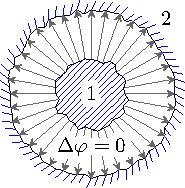
\includegraphics[scale=1.5]{img/lect4_ris4}
	\caption{Закрытая линия из двух проводников}
	\label{fig:lect4:4}
\end{figure}

Можно модифицировать задачу с нитью, если сделать нити две (рис. \ref{fig:lect4:5}):

\begin{figure}[H]
	\centering
	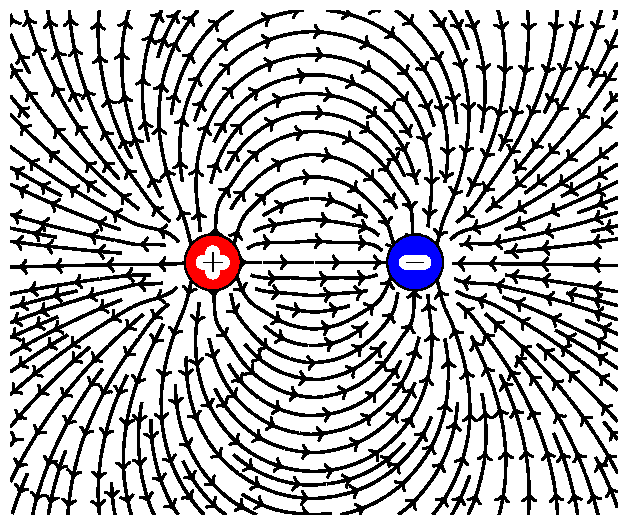
\includegraphics[scale=0.7]{img/lect4_ris5}
	\caption{Поле двухпроводной линии}
	\label{fig:lect4:5}
\end{figure}

В поперечном разрезе это поле диполя, а оно спадает быстрее, $\sim \frac{1}{r^2}$. Тогда
\begin{equation}
	E_\perp\sim H_\perp \sim \frac{1}{r^2}
	\quad \Rightarrow \quad
	\overline{S}_z \sim \frac{1}{r^4}, \quad
	\Pi \sim \int\limits_{L_\text{характ}}^\infty \frac{1}{r^3} \dd{r}
\end{equation}

Мощность волны получится уже конечным числом, значит, в модифицированной задаче TEM-волна энергетически реализуема.

\textbf{Конечный вывод:} TEM-волна в идеальной линии передачи возможна, если число проводников $\geq 2$.

Например, в коаксиальной линии (рис. \ref{fig:lect4:6}) TEM-волна возможна.

\begin{figure}[H]
	\centering
	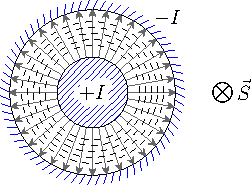
\includegraphics[scale=1.5]{img/lect4_ris6}
	\caption{Поле в коаксиальном кабеле}
	\label{fig:lect4:6}
\end{figure}

Зададимся вопросом: возможны ли в такой линии TE и TM волны? Сформулируем утверждение, пока без доказательства: \textbf{в открытых линиях передачи TE и TM волны не существуют}.

\subsection{TE и TM волны в идеальных линиях передачи закрытого типа}


\subsubsection{TE и TM волны в прямоугольном волноводе}

\paragraph{Решение для TM-волн.} Займемся решением TM-волны в прямоугольном волноводе (рис. \ref{fig:lect4:7}). Условимся что $a>b$. Эта задача поиска собственных функций $\phi^e$ и собственных значений $\varkappa$:
\begin{equation}
	\Delta_\perp \phi^e+\kappa^2\phi^e=0, \quad \phi^e|_l=0
\end{equation}

\begin{figure}[h!]
	\centering
	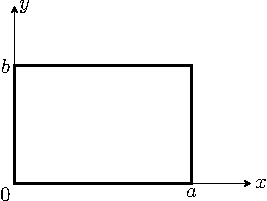
\includegraphics[scale=1.5]{img/lect4_ris7}
	\caption{Прямоугольный волновод}
	\label{fig:lect4:7}
\end{figure}

В матфизике эта задача о колебании мембраны с закрепленным краем. Она решается разделением переменных:
\begin{equation}
	\phi^e=X(x)\cdot Y(y)
\end{equation}
\begin{equation}
	\pdv[2]{\phi^e}{x}
		+\pdv[2]{\phi^e}{y}
			+\kappa^2 \phi^e =0  \quad \bigg| \cdot \frac{1}{XY}
	\quad \Rightarrow \quad
		\frac{X''}{X}+\frac{Y''}{Y}+\varkappa^2=0
\end{equation}

Тут надо произнести магическую фразу: так как первое слагаемое функция от $x$, второе функция от $y$, и их сумма равна константе для любых $x,y$, значит -- сами слагаемые тоже какие-то константы:
\begin{equation}
	\frac{X''}{X}=-\kappa_x^2, \quad
	\frac{Y''}{Y}=-\kappa_y^2
\end{equation}
Определив таким образом константы, мы получаем:
\begin{equation}
	\kappa_x^2+ \kappa_y^2=\kappa^2
\end{equation}
Пока мы не нашли само $\kappa$. Это собственное число, и оно подлежит определению. Прежде чем его найти, найдем собственные функции, решая уравнения
\begin{equation}
	X''+\kappa_x^2X=0, \quad Y''+\kappa_y^2Y=0
\end{equation}	
Это уравнения известного вида, их решение
\begin{equation}
	X=C_1\cdot\cos{\kappa_x x}+
		C_2\cdot\sin{\kappa_x x}
	\qquad
	Y=A_1\cdot\cos{\kappa_y y}+
		A_2\cdot\sin{\kappa_y y}	
\end{equation}
Нужно удовлетворить граничным условиям: 
\begin{equation}
	\phi^e|_{y=0}=0 \quad \Rightarrow \quad
		X(x)Y(0)=0 \quad \forall x \Rightarrow
		Y(0)=0 \quad \Rightarrow \quad A_1=0
\end{equation}
\begin{equation}
	\phi^e|_{x=0}=0 \quad \Rightarrow \quad
		X(0)Y(y)=0 \quad \forall y \Rightarrow
		X(0)=0 \quad \Rightarrow \quad C_1=0
\end{equation}
\begin{gather}
	\phi^e|_{x=a}=0 \quad \Rightarrow \quad
		X(a)Y(y)=0 \quad \forall y  \Rightarrow  \\ \Rightarrow
		X(a)=0 \quad \Rightarrow \quad \kappa_x a = m\pi, \quad m=\xcancel{0},1,2,\ldots
\end{gather}
Поскольку $m=0$ дает тривиальное решение, мы его откидываем.
\begin{gather}
	\phi^e|_{y=b}=0 \quad \Rightarrow \quad
		X(x)Y(b)=0 \quad \forall x  \Rightarrow  \\ \Rightarrow
		Y(b)=0 \quad \Rightarrow \quad \kappa_y b = n\pi , \quad n=\xcancel{0},1,2,\ldots
\end{gather}
Теперь мы получили выражения для $X$ и $Y$:
\begin{gather}
	X_m(x)=C_2\cdot\sin\frac{\pi m x}{a}\\
	Y_n(x)=A_2\cdot\sin\frac{\pi n y}{b}
\end{gather}
Теперь можем окончательно записать выражения для собственных функций и собственных значений в решении TM-волн:
\begin{gather}
	\label{phi_tm}
	\left.\begin{aligned}
		&\phi^e_{mn}=B_{mn}\sin\frac{\pi m x}{a}\sin\frac{\pi n y}{b}\\
		&\kappa_{mn}^2=\qty(\frac{m\pi}{a})^2+\qty(\frac{n\pi}{b})^2	
	\end{aligned}\right\}\,, \quad m,n=1,2,\ldots
\end{gather}
\paragraph{Решение для TE-волн.} Приведем решение без вывода:
\begin{gather}
	\label{phi_te}
	\left.\begin{aligned}
		&\phi^m_{mn}=B_{mn}\cos\frac{\pi m x}{a}\cos\frac{\pi n y}{b}\\
		&\kappa_{mn}^2=\qty(\frac{m\pi}{a})^2+\qty(\frac{n\pi}{b})^2	
	\end{aligned}\right\}\,, \quad m,n=(0),1,2,\ldots
\end{gather}
Важным отличием является то, что теперь одно из чисел $m,n$ может быть равно нулю (решение от этого не станет тривиальным).

\paragraph{Низшая мода.} По определению, низшая мода -- та, у которой минимальное поперечное волновое число. Так как мы предполагали, что $a>b$, то в нашем случае это мода TE$_{10}$:
\begin{equation}
	\kappa_{10}=\frac{\pi}{a} \quad \rightarrow \quad \omega_{cr\,10}=\frac{\kappa_{10}\cdot c}{\sqrt{\varepsilon \mu}} 	
\end{equation} 

Именно моду TE$_{10}$ чаще всего используют на практике в линиях передачи. 

Рассмотрим перпендикулярную структуру поля TE$_{10}$-волны. Нарисуем силовые линии полей $E$ и $H$ в плоскости $(x,y)$ -- перпендикулярной распространению волны (рис. \ref{fig:lect4:8})
\begin{figure}[h!]
	\centering
	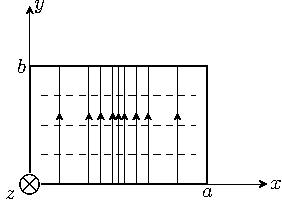
\includegraphics[scale=1.5]{img/lect4_ris8}
	\caption{Структура полей $\vec{E}$ и $\vec{H}$ ($\vec{H}$ изображено пунктиром)}
	\label{fig:lect4:8}
\end{figure}

На границах волновода поле $E$ равно нулю (в силу условия $E_\tau=0$). Поле $\vec{E}$ можем получить из уравнений \eqref{phi_te},\eqref{eperp}:
\begin{equation}
	\vec{E}=\vec{E}_\perp=\vec{y}_0E_0\cdot\sin\frac{\pi x}{a}\exp[i(\omega t - hz)],
\end{equation}
где 
\begin{equation}
	h=\sqrt{
		\frac{\omega^2}{c^2}\epsilon \mu - \qty(\frac{\pi}{a})^2
	}
\end{equation}

Поле $H$ можно найти из импедансного соотношения (для TE-волны):
\begin{equation}
	\frac{E_y}{H_x}=-\sqrt\frac{\mu}{\epsilon}\frac{k}{h}
\end{equation}

\begin{figure}[h!]
	\centering
	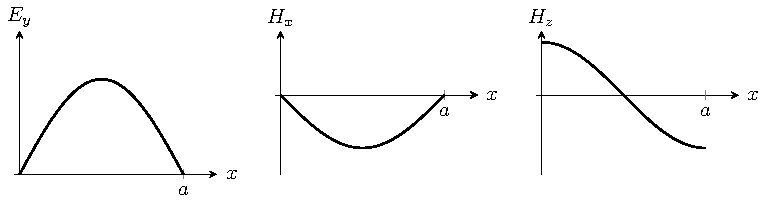
\includegraphics[width=\textwidth]{img/lect4_ris9}
	\caption{Поперечная структура полей $\vec{E}$ и $\vec{H}$ (мода TE$_{}$)}
	\label{fig:lect4:9}
\end{figure}

За перенос энергии отвечают именно поперечные компоненты поля. Компонента поля
$H_z \sim \cos\frac{\pi a}{x}$ также сдвинута по фазе во времени. 

\begin{figure}[H]
	\centering
	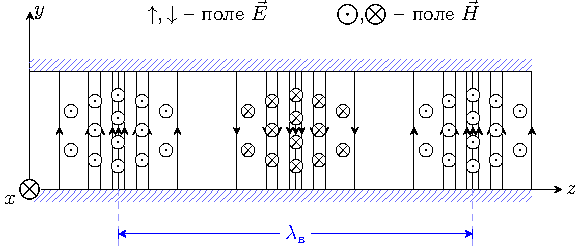
\includegraphics[width=\textwidth]{img/lect4_ris10}
	\caption{Продольная структура полей $\vec{E}$ и $\vec{H}$ (мода TE$_{}$)}
	\label{fig:lect4:10}
\end{figure}

\begin{figure}[H]
	\centering
	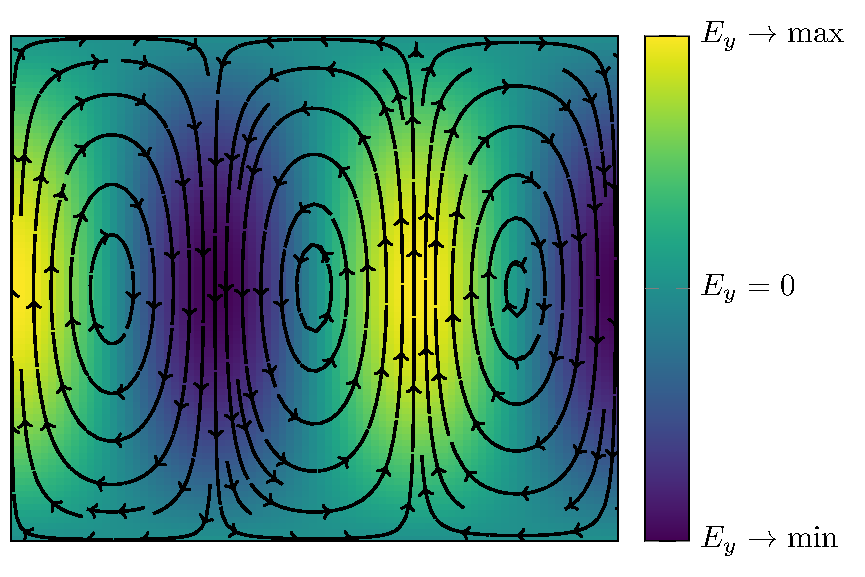
\includegraphics[scale=1]{img/lect4_ris11}
	\caption{Структура поля $\vec{H}$ (изображены силовые линии) и поля $\vec{E}$ (напряженность изображена цветом) волны TE$_{10}$ в прямоугольном волноводе}
	\label{fig:lect4:11}
\end{figure}

\paragraph{Высшие моды.} В зависимости от соотношения между $a$ и $b$, порядок мод может быть разным (он определяется величиной поперечного волнового числа). Некоторые высшие моды:
\begin{equation}
\begin{aligned}
 		\text{TE}_{11}:& \quad  \kappa_{11}=\sqrt{\qty(\frac{\pi}{a})^2+\qty(\frac{\pi}{b})^2}\\
 		\text{TE}_{20}:& \quad  \kappa_{20}=\frac{2\pi}{a} \\
 		\text{TE}_{01}:& \quad  \kappa_{11}=\frac{\pi}{b}
\end{aligned} 	
\end{equation} 

\paragraph{Мода TE$_{11}$.} В волне TE$_{11}$ $\kappa_{11}=\sqrt{\qty(\frac{\pi}{a})^2+\qty(\frac{\pi}{b})^2}$
\begin{figure}[H]
	\centering
	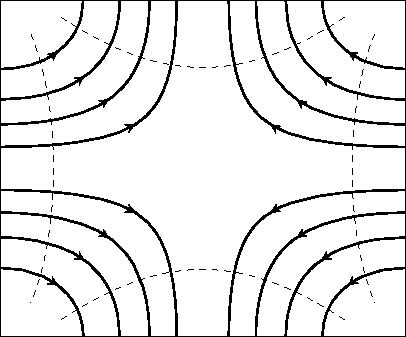
\includegraphics[scale=1.5]{img_lect5/rectangle/TE11}
	\caption{Электрическое и магнитное поле в волне TE$_{11}$}
	\label{fig:rectangle:TE11}
\end{figure}
Такую структуру поля называют <<розеткой>>.

\paragraph{Мода TE$_{mn}$.} А что будет, если мы посмотрим на структуру поля, например, TE$_{2019,1938}$? Для мод высоких порядков $m>1, n>1$, нужно разделить волновод на $m$ частей по горизонтали и $n$ по вертикали, и в каждой такой ячейке поле будет повторять структуру моды TE$_{11}$. При этом направление силовых линий в соседних ячейках должно быть согласовано.

Пример структуры поля приведен на рисунке \ref{fig:rectangle:TE44}, для случая $m=n=4$.
\begin{figure}[H]
	\centering
	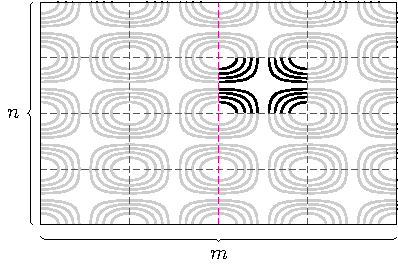
\includegraphics[scale=1.5]{img_lect5/rectangle/TE44}
	\caption{Электрическое поле в волне TE$_{44}$}
	\label{fig:rectangle:TE44}
\end{figure}

Перейдем к описанию TM-волн.

\paragraph{Мода TM$_{11}$.} Для волн в прямоугольном волноводе $\kappa_{mn}^{(TE)}=\kappa_{mn}^{(TM)}$, т.е. существует хотя бы двукратное вырождение волнового числа: одному волновому числу соответствует несколько мод.
\begin{figure}[H]
	\centering
	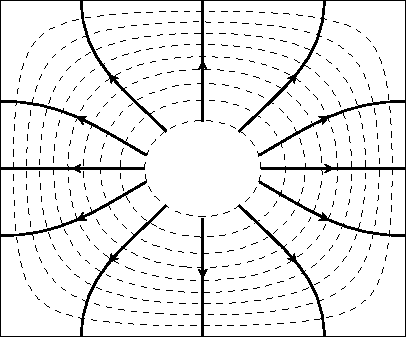
\includegraphics[scale=1.5]{img_lect5/rectangle/TM11}
	\caption{Электрическое и магнитное поле в волне TM$_{11}$}
	\label{fig:rectangle:TM11}
\end{figure}



\paragraph{Мода TM$_{21}$.} Аналогично моде TE$_{mn}$, для мод TM$_{mn}$ нужно разделить волновод на $m$ частей по горизонтали и $n$ по вертикали, и в каждой такой ячейке поле будет повторять структуру моды TM$_{11}$. При этом направление силовых линий в соседних ячейках должно быть согласовано.
\begin{figure}[H]
	\centering
	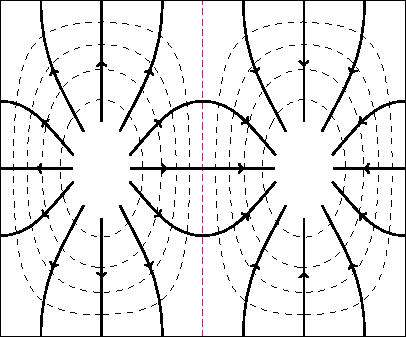
\includegraphics[scale=1.5]{img_lect5/rectangle/TM21}
	\caption{Электрическое и магнитное поле в волне TM$_{21}$}
	\label{fig:rectangle:TM21}
\end{figure}

Заметим, что линии электрического поля входят в стенки волновода под прямым углом. Иначе и быть не может, в силу граничного условия на проводнике $E_\tau=0$.

\subsubsection{TE и TM волны в круглом волноводе}

Наиболее часто на практике используются прямоугольные, круглые и коаксиальные волноводы. Займемся изучением круглых волноводов.

\begin{figure}[ht]
	\centering
	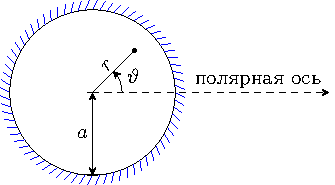
\includegraphics[scale=1.65]{img_lect5/cylindric/geometry}
	\caption{Геометрия круглого волновода}
	\label{fig:cylinder:geometry}
\end{figure}

Область определения задачи $0\leq r \leq a$, $0\leq \vartheta \leq 2\pi$. Каждая точка в сечении волновода задается двумя координатами $(r,\vartheta)$.

Будем решать задачу (пока в общем виде, без граничных условий):
\begin{equation}
	\Delta_\perp \phi+\kappa^2\phi=0
\end{equation}

Здесь лаплассиан в цилиндрических координатах
\begin{equation}
	\Delta_\perp\phi=\frac{1}{r}\pdv{r}\qty(r\pdv{\phi}{r})+\frac{1}{r^2}\pdv[2]{\phi}{\vartheta}
\end{equation}

Также как и при поиске поля в прямоугольном волноводе, воспользуемся методом разделения переменных:
\begin{equation}
	\phi=R(r)\cdot\Theta(\vartheta)
\end{equation}

Применив стандартным образом разделение переменных (подставив $\phi$ как $R\cdot\Theta$ в решаемое уравнение и домножив уравнение слева и справа на $\frac{r^2}{R\Theta}$), получим
\begin{equation}
	\underbrace{r^2\frac{R''}{R}+r\frac{R'}{R}+\kappa^2r^2}_{f(r)=+C_1}+
	\underbrace{\frac{\Theta''}{\Theta}}_{g(\vartheta)=-C_1}
	=0
\end{equation}

Заметим, что комбинация из первых трех слагаемых может зависеть только от $r$, последнее слагаемое может зависеть только от $\vartheta$, а их сумма ни от чего не зависит - значит и первые три слагаемых в сумме ни от чего не зависят и равны некой константе $-C_1$, тогда последнее слагаемое (которое тоже ни от чего не зависит) равно $+C_1$.

Таким образом, разделение переменных успешно завершилось.
\paragraph{Уравнение относительно $\Theta$.}
Такое уравнение запишется в виде
\begin{equation}
	\Theta''+C_1\Theta=0
\end{equation}
Решение этого уравнения (гармонического осциллятора) нам хорошо известно:
\begin{equation}
	\Theta=A_1\cos(\sqrt{C_1}\vartheta)+A_2\sin(\sqrt{C_1}\vartheta)
\end{equation}
Сразу заметим, что отсюда следует, что $\sqrt{C_1}=m$ -- целое число. Действительно, в силу симметрии задачи
\begin{equation}
	\Theta(\vartheta)=\Theta(\vartheta+2\pi),
\end{equation}
а такое возможно только при целой частоте $\sqrt{C_1}$.

\paragraph{Уравнение относительно $r$.} Его можно переписать, если учесть что $\sqrt{C_1}=m$, тогда
\begin{equation}
	R''+\frac{1}{r}R'+\qty(\kappa^2-\frac{m^2}{r^2})R=0
\end{equation}
Можно ввести замену переменных $x=\kappa r$, тогда
\begin{equation}
	R''_{xx}+\frac{1}{x}R'_x+\qty(1-\frac{m^2}{x^2})R=0, \quad R=R(x)
\end{equation}
Это известное уравнение Бесселя. Его решение получается в виде специальных, цилиндрических функций Бесселя:
\begin{equation}
	R=B_q\cdot J_m(x)+B_2\cdot N_m(x)
\end{equation}
$J_m$ называют функциями Бесселя первого рода, или просто функциями Бесселя, а $N_m$ функциями Бесселя второго рода, или функциями Неймана. Их поведение хорошо изучено, не хуже чем поведение синуса и косинуса. Рассмотрим некоторые характерные моменты.
\begin{figure}[ht]
	\centering
	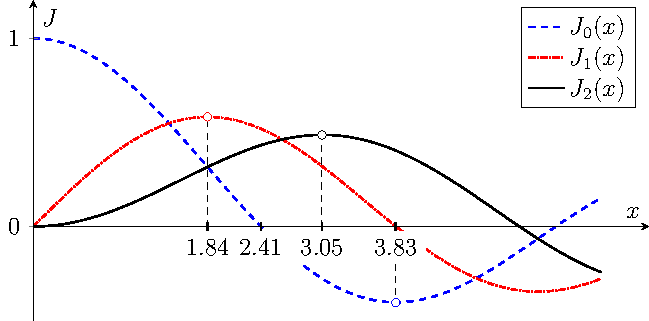
\includegraphics[scale=1.3]{img_lect5/bessel/bessel012}
	\caption{Функции Бесселя первого рода}
	\label{fig:cylinder:besselJ}
\end{figure}
Первый максимум функции Бесселя второго порядка лежит на пересечении функций Бесселя первого и нулевого порядков. Это свойство функций Бесселя. Еще одно свойство заключается в том, что ноль функции Бесселя первого порядка совпадает с точкой минимума функции Бесселя нулевого порядка.
\begin{figure}[ht]
	\centering
	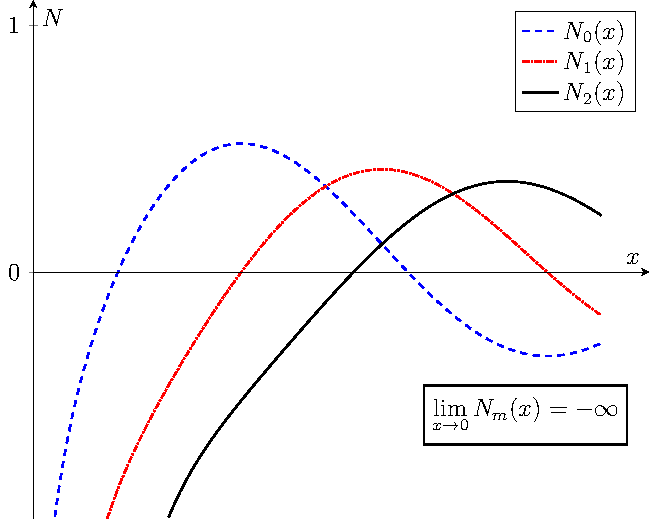
\includegraphics[scale=1.4]{img_lect5/bessel/besselY012}
	\caption{Функции Бесселя второго рода}
	\label{fig:cylinder:besselN}
\end{figure}
Функции Неймана мы пока не будем рассматривать подробно. Это вызвано тем, что у всех функций Неймана есть особенность: в нуле они расходятся, и поэтому в нашем решении, чтобы решение в нуле было конечно, придется положить $B_2=0$.

Вообще говоря, в коаксиальной линии это будет не так, потому что там область определения задачи не включает $r=0$, и  будет $B_2\ne0$.

Итак, наше решение теперь можно переписать в виде
\begin{equation}
	\phi_m=J_m(\kappa r)\qty(A_1\cos(m \vartheta)+A_2\sin(m \vartheta))
\end{equation}
Здесь константу $B_1$ мы уже не пишем, предпологая что она сидит в константах $A_1,A_2$.
Иногда, для краткости, комбинацию синуса и косинуса пишут так:
\begin{equation}
	A_1\cos(m \vartheta)+A_2\sin(m \vartheta)=\mqty(\cos m\vartheta \\\sin m\vartheta)
\end{equation}

Перейдем к удовлетворению граничных условий.

\paragraph{Граничные условия TE-волн.} На границе волновода должна занулятся производная поперечной функции:
\begin{equation}
	\pdv{\phi}{r}\bigg|_{r=a}=0 \quad \Rightarrow \quad \pdv{J_m(\kappa r)}{r}\bigg|_{r=a}=0
\end{equation}
Это значит, что
\begin{equation}
	J_m'(x)=0, \quad x=\kappa a
\end{equation}
Мы можем пронумеровать все нули производной, и обозначить эти точки $x=\mu_{mn}$, где $m$ -- порядок функции Бесселя, а $n$ -- номер нуля производной. Например, $\mu_{11}=1.84$. 
\begin{figure}[H]
	\centering
	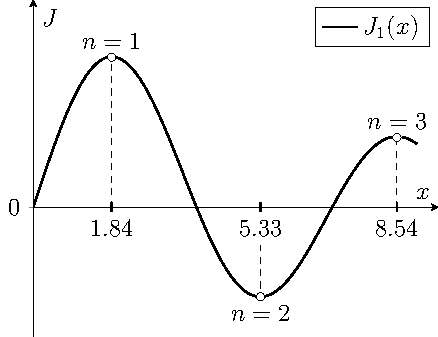
\includegraphics[scale=1.4]{img_lect5/bessel/bessel_mu}
	\caption{Нули производной функции Бесселя}
	\label{fig:cylinder:besselN}
\end{figure}
Тогда можем выразить через $\mu$ и волновое число:
\begin{equation}
	\kappa_{mn}^{TE}=\frac{\mu_{mn}}{a}
\end{equation}
В итоге получаем решение для TE-волн:
\begin{equation}
	\phi_m=C_{mn} J_m(\kappa_{mn} r)\mqty(\cos m\vartheta \\\sin m\vartheta), \quad
	m=0,1,2,3,\ldots \quad n=1,2,\ldots
\end{equation}
Некоторые значения:
\begin{equation}
\begin{aligned}
 		\mu_{11}=&1.84, \quad \kappa_{11}=&\frac{1.84}{a}\\[0.7em]
 		\mu_{21}=&3.05, \quad \kappa_{21}=&\frac{3.05}{a}\\[0.7em]
 		\mu_{01}=&3.83, \quad \kappa_{01}=&\frac{3.83}{a}
\end{aligned} 	
\end{equation} 
\paragraph{Граничные условия TM-волн.} Теперь на границе зануляется поперечная функция:
\begin{equation}
	\phi\big|_{r=a}=0 
		\quad \Rightarrow \quad
			J_m(\kappa r)=0
\end{equation}
Также, как мы это делали для TE-волн, пронумеруем нули функции Бесселя:
\begin{figure}[H]
	\centering
	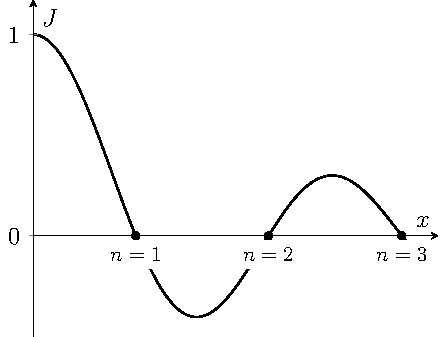
\includegraphics[scale=1.5]{img_lect5/bessel/bessel_kappa}
	\caption{Нули функции Бесселя}
	\label{fig:cylinder:besselN}
\end{figure}
И обозначим нули 
\begin{equation}
	x=\nu_{mn},
\end{equation}
И тогда
\begin{equation}
	\kappa_{mn}^{TM}=\frac{\nu_{mn}}{a}
\end{equation}

Некоторые значения:
\begin{equation}
\begin{aligned}
 		\nu_{01}=&2.405, \quad \kappa_{01}^{TM}=&\frac{2.405}{a}\\[1em]
 		\mu_{11}=&3.83, \quad \kappa_{11}^{TM}=&\frac{3.83}{a}
\end{aligned} 	
\end{equation}

\paragraph{Полное решение задачи.} Если мы введем волновое число как
\begin{equation}
	\kappa_{mn}=\left\{
	\begin{aligned}
		\frac{\mu_{mn}}{a}, \quad \mathrm{TE},\\
		\frac{\nu_{mn}}{a}, \quad \mathrm{TM}
	\end{aligned}\right.
\end{equation}
Тогда полное решение задачи запишется  в виде
\begin{equation}
	\phi_m=C_{mn} J_m(\kappa_{mn} r)\mqty(\cos m\vartheta \\\sin m\vartheta), \quad
	m=0,1,2,3,\ldots \quad n=1,2,\ldots
\end{equation}
\paragraph{Низшая мода.} У низшей моды наименьшее волновое число. В случае круглого волновода низшей модой будет TE$_{11}$: $\kappa_{11}=\frac{1.84}{a}$.
\begin{figure}[H]
	\centering
	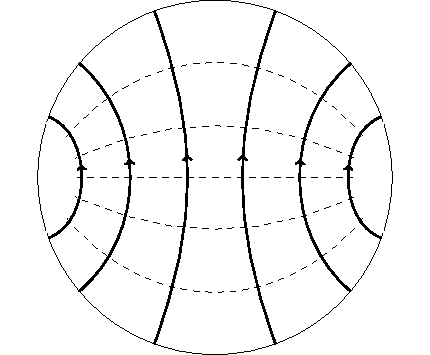
\includegraphics[scale=1.4]{img_lect5/cylindric/TE11}
	\caption{Электрическое и магнитное поле в волне TE$_{11}$}
	\label{fig:cylinder:TE11}
\end{figure}
\paragraph{Замечание.} Можно сформулировать некоторое правило рисования силовых линий. Если построить линии уровня $\phi=\mathrm{const}$, то это будут силовые линии чисто поперечного поля.

Вообще говоря, поле моды TE$_{11}$ круглого волновода топологически подобно моде TE$_{10}$ прямоугольного волновода. Если постепенно деформировать стенки прямоугольного волновода, скругляя их, то линии поля постепенно будут переходить в линии поля круглого волновода.
\begin{figure}[H]
	\centering
	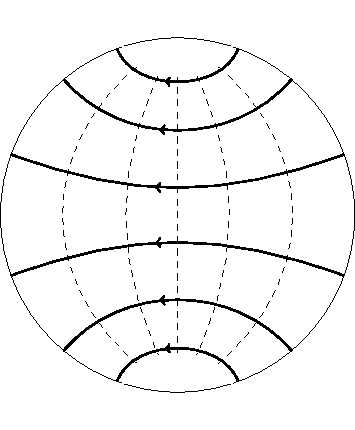
\includegraphics[scale=1.4]{img_lect5/cylindric/TE11_rotated}
	\caption{Поляризационное вырождение моды TE$_{11}$}
	\label{fig:cylinder:TE11_rotated}
\end{figure}
Кроме того, мода TE$_{11}$ круглого волновода \textbf{двукратно вырождена:} имеет место так называемое \textbf{поляризационное вырождение} (рис. \ref{fig:cylinder:TE11_rotated}).

Действительно, если повернуть волновод на 90 градусов, то получаем другое решение. Их не бесконечно много, а всего два фундаментальных, а все остальные образуются как их суперпозиция. 


Перейдем к рассмотрению следующих (по росту волнового числа) волн.
\newpage
\paragraph{Мода TM$_{01}$.} Вообще говоря, волны с первым индексом $0$ TE$_{0n}$, TM$_{0n}$ не зависят от координат и называются \textbf{симметричными модами.}
\begin{figure}[H]
	\centering
	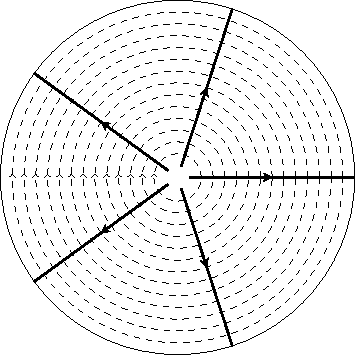
\includegraphics[scale=1.25]{img_lect5/cylindric/TM01}
	\caption{Электрическое и магнитное поле в волне TM$_{01}$}
	\label{fig:cylinder:TM01}
\end{figure}

\begin{figure}[H]
	\centering
	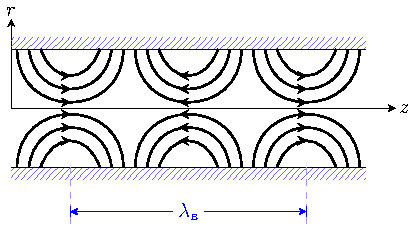
\includegraphics[scale=2]{img_lect5/cylindric/TM01z}
	\caption{Вид в продольном разрезе на волну TM$_{01}$}
	\label{fig:cylinder:TM01}
\end{figure}

\newpage
\paragraph{Мода TE$_{21}$.} $\kappa_{21}=\frac{3.05}{a}$
\begin{figure}[H]
	\centering
	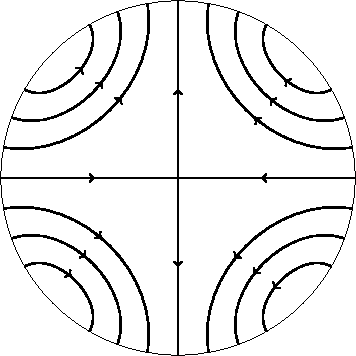
\includegraphics[scale=1.5]{img_lect5/cylindric/TE21}
	\caption{Электрическое поле в волне TE$_{21}$}
	\label{fig:cylinder:TE21}
\end{figure}

\paragraph{Мода TE$_{01}$.} $\kappa_{01}^{TE}=\kappa_{11}^{TM}=\frac{3.83}{a}$
\begin{figure}[H]
	\centering
	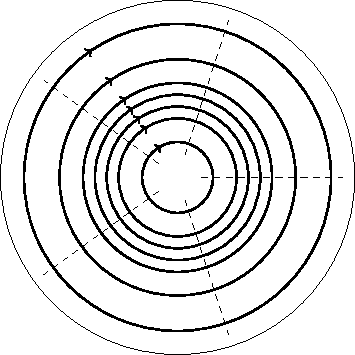
\includegraphics[scale=1.5]{img_lect5/cylindric/TE01}
	\caption{Электрическое и магнитное поле в волне TE$_{01}$}
	\label{fig:cylinder:TE01}
\end{figure}
\newpage
\paragraph{Мода TM$_{11}$.} $\kappa_{01}^{TE}=\kappa_{11}^{TM}=\frac{3.83}{a}$
\begin{figure}[H]
	\centering
	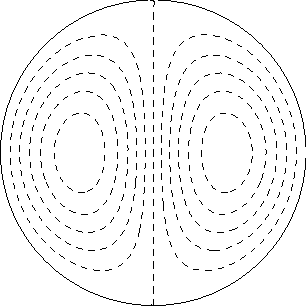
\includegraphics[scale=1.5]{img_lect5/cylindric/TM11}
	\caption{Магнитное поле в волне TM$_{11}$}
	\label{fig:cylinder:TM11}
\end{figure}

\paragraph{Высокая мода TM$_{81}$.} Первый индекс определяет изрезанность по углу: 
\begin{figure}[H]
	\centering
	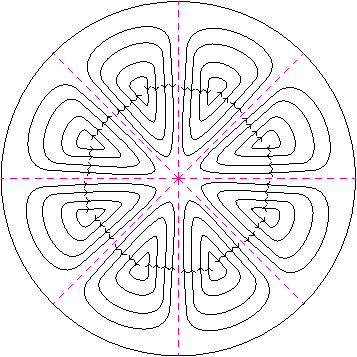
\includegraphics[scale=1.5]{img_lect5/cylindric/TM81}
	\caption{Магнитное поле в волне TM$_{81}$}
	\label{fig:cylinder:TM81}
\end{figure}

\newpage
\paragraph{Высокая мода TE$_{m1}$, $m\geq 1$.} Эту моду можно описать и на языке геометрической оптики. Её также называют модой шепчущей галереи.
\begin{figure}[H]
	\centering
	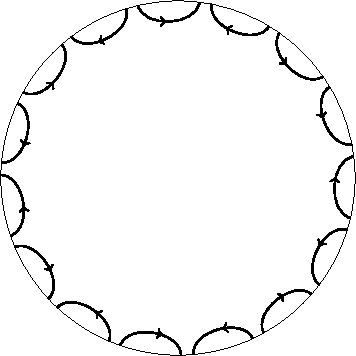
\includegraphics[scale=1.5]{img_lect5/cylindric/TEm1}
	\caption{Электрическое поле в волне TE$_{m1}$}
	\label{fig:cylinder:TMm1}
\end{figure}

Шепчущая галерея - это многократное переотражение волны вдоль стенки. Если два монаха стоят на противоположных концах диаметра, а настоятель в центре, то он не слышит разговор монахов, а они друг друга слышат: волна распространяется, двигаясь под малым углом к стене.
 % Лекция от 27.02
\newpage
%!TEX root = ../lections.tex
\subsection{Главные (TEM) волны в линиях передачи с идеальными границами}

У TEM-волн поперечное волновое число $\varkappa=0$:
\begin{equation}
	\varkappa=0 \Rightarrow h=k= \frac{\omega}{c}\sqrt{\varepsilon \mu}
\end{equation}
Поля таких волн выражаются следующим образом через функцию $\varphi$:
\begin{gather}
	\label{eperp}
	\vec{E}_\perp=-\frac{1}{\sqrt{\varepsilon \mu}}\nabla_\perp \varphi\\
	\vec{E}_\perp=-\frac{1}{\mu}\qty[\nabla_\perp \varphi,\vec{z}_0]
\end{gather}

При этом выполняются \textbf{граничные условия}: на каждом из проводников (допустим, есть набор проводников, вдоль которых распространяется волна)
\begin{equation}
	\varphi|_{l_i}=C_i,
\end{equation}
причем константа не обязана быть одна для всех проводников.

\begin{figure}[H]
	\centering
	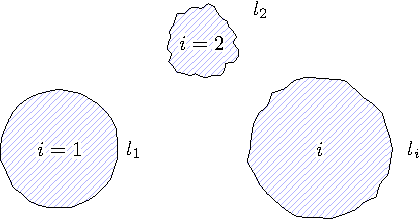
\includegraphics[scale=1.5]{img/lect4_ris1}
	\caption{Набор проводников в задаче}
	\label{fig:lect4:1}
\end{figure}

\subsubsection{Внутренняя задача}
\begin{figure}[H]
	\centering
	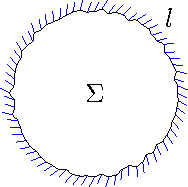
\includegraphics[scale=1.5]{img/lect4_ris2}
	\caption{Случай одного проводника}
	\label{fig:lect4:2}
\end{figure}
Пусть у нас есть только один проводник, в котором есть цилиндрическая полость (рис. \ref{fig:lect4:2}). Рассмотрим внутреннюю задачу, т.е. распространение волны внутри цилиндрической полости. Оказывается, для граничного условия $\varphi_\perp|_l=C_1$ существует только тривиальное решение $\varphi_\perp=C_1$. В матфизике это доказывается. Начало доказательства такое:

\begin{equation}
	\Delta \varphi=\Div\qty(\varphi\nabla \varphi)=0 \quad \bigg| \iint\limits_\Sigma
\end{equation}
Это такая задача, которую проще доказать самому. Попробуйте это сделать сами.

\subsubsection{Внешняя задача}
Зададимся вопросом о решении той же задачи:
\begin{equation}
	\Delta_\perp \varphi=0, \quad \varphi|_l=\mathrm{const}
\end{equation}
Только теперь будем рассматривать её в области вне проводника, т.н. внешняя задача.

Для начала рассмотрим задачу попроще, поле нити (рис. \ref{fig:lect4:3}). Решение её известно:
\begin{equation}
 	\Delta_\perp \varphi=0 
 		\quad \Rightarrow \quad
 	\varphi \sim \ln r
\end{equation} 

Характер убывания полей здесь $E_r\sim \frac{1}{r}$, а для магнитного поля в силу импедансного соотношения $\frac{E_r}{H_\phi}=\eta_{\perp\text{в}}=1$ $H_\varphi\sim\frac{1}{r}$:
\begin{equation}
	E_r=H_\phi\sim\frac{1}{r}
\end{equation}
\begin{figure}[h!]
	\centering
	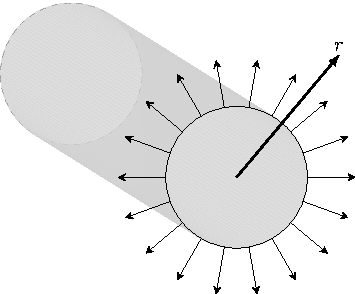
\includegraphics[scale=1.5]{img/lect4_ris3}
	\caption{Поле бесконечной проводящей нити}
	\label{fig:lect4:3}
\end{figure}

Посмотрим на поведение полей при $r\to\infty$. Говорят, нужно поставить граничные условия (или закон убывания) на бесконечности. Чем плох закон $\frac{1}{r}$?

Посчитаем средний по времени поток энергии через поперечное сечение, в котором распространяется волна. Сечение бесконечно, за исключением конечной площади проводника.

Сначала вычислим вектор Пойнтинга (средний по времени и в проекции на $z$):
\begin{equation}
	\overline{S}_z=\frac{c}{8 \pi}\mathrm{Re}\qty(E_r\cdot H_\phi^*)\sim\frac{1}{r^2}
\end{equation}
\begin{equation}
	\Pi=\iint\limits_\Sigma \overline{S}_z ds \sim
	\iint\limits_\Sigma \frac{1}{r^2} (2\pi r \dd{r})
	\sim \int\limits_a^\infty = \ln\frac{\infty}{a}=\infty
\end{equation}
Интеграл расходится на бесконечности. Говорят, что расходимость носит логарифмический характер. Получили бесконечную мощность волны: такую волну невозможно создать реальным источником --- волна не удовлетворяет критерию энергетической реализуемости.

Можно сделать важный вывод: \textbf{вдоль одиночного проводника TEM-волна с конечной энергией распространятся не может}. А может,если проводников больше. Например, в линии из двух проводников (рис. \ref{fig:lect4:4}) TEM-волна уже возможна.

\begin{figure}[H]
	\centering
	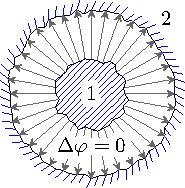
\includegraphics[scale=1.5]{img/lect4_ris4}
	\caption{Закрытая линия из двух проводников}
	\label{fig:lect4:4}
\end{figure}

Можно модифицировать задачу с нитью, если сделать нити две (рис. \ref{fig:lect4:5}):

\begin{figure}[H]
	\centering
	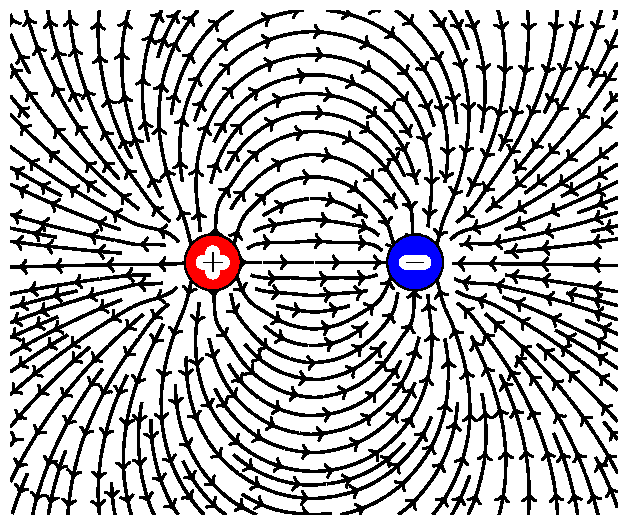
\includegraphics[scale=0.7]{img/lect4_ris5}
	\caption{Поле двухпроводной линии}
	\label{fig:lect4:5}
\end{figure}

В поперечном разрезе это поле диполя, а оно спадает быстрее, $\sim \frac{1}{r^2}$. Тогда
\begin{equation}
	E_\perp\sim H_\perp \sim \frac{1}{r^2}
	\quad \Rightarrow \quad
	\overline{S}_z \sim \frac{1}{r^4}, \quad
	\Pi \sim \int\limits_{L_\text{характ}}^\infty \frac{1}{r^3} \dd{r}
\end{equation}

Мощность волны получится уже конечным числом, значит, в модифицированной задаче TEM-волна энергетически реализуема.

\textbf{Конечный вывод:} TEM-волна в идеальной линии передачи возможна, если число проводников $\geq 2$.

Например, в коаксиальной линии (рис. \ref{fig:lect4:6}) TEM-волна возможна.

\begin{figure}[H]
	\centering
	\includegraphics[scale=1.5]{img/lect4_ris6}
	\caption{Поле в коаксиальном кабеле}
	\label{fig:lect4:6}
\end{figure}

Зададимся вопросом: возможны ли в такой линии TE и TM волны? Сформулируем утверждение, пока без доказательства: \textbf{в открытых линиях передачи TE и TM волны не существуют}.

\subsection{TE и TM волны в идеальных линиях передачи закрытого типа}


\subsubsection{TE и TM волны в прямоугольном волноводе}

\paragraph{Решение для TM-волн.} Займемся решением TM-волны в прямоугольном волноводе (рис. \ref{fig:lect4:7}). Условимся что $a>b$. Эта задача поиска собственных функций $\phi^e$ и собственных значений $\varkappa$:
\begin{equation}
	\Delta_\perp \phi^e+\kappa^2\phi^e=0, \quad \phi^e|_l=0
\end{equation}

\begin{figure}[h!]
	\centering
	\includegraphics[scale=1.5]{img/lect4_ris7}
	\caption{Прямоугольный волновод}
	\label{fig:lect4:7}
\end{figure}

В матфизике эта задача о колебании мембраны с закрепленным краем. Она решается разделением переменных:
\begin{equation}
	\phi^e=X(x)\cdot Y(y)
\end{equation}
\begin{equation}
	\pdv[2]{\phi^e}{x}
		+\pdv[2]{\phi^e}{y}
			+\kappa^2 \phi^e =0  \quad \bigg| \cdot \frac{1}{XY}
	\quad \Rightarrow \quad
		\frac{X''}{X}+\frac{Y''}{Y}+\varkappa^2=0
\end{equation}

Тут надо произнести магическую фразу: так как первое слагаемое функция от $x$, второе функция от $y$, и их сумма равна константе для любых $x,y$, значит -- сами слагаемые тоже какие-то константы:
\begin{equation}
	\frac{X''}{X}=-\kappa_x^2, \quad
	\frac{Y''}{Y}=-\kappa_y^2
\end{equation}
Определив таким образом константы, мы получаем:
\begin{equation}
	\kappa_x^2+ \kappa_y^2=\kappa^2
\end{equation}
Пока мы не нашли само $\kappa$. Это собственное число, и оно подлежит определению. Прежде чем его найти, найдем собственные функции, решая уравнения
\begin{equation}
	X''+\kappa_x^2X=0, \quad Y''+\kappa_y^2Y=0
\end{equation}	
Это уравнения известного вида, их решение
\begin{equation}
	X=C_1\cdot\cos{\kappa_x x}+
		C_2\cdot\sin{\kappa_x x}
	\qquad
	Y=A_1\cdot\cos{\kappa_y y}+
		A_2\cdot\sin{\kappa_y y}	
\end{equation}
Нужно удовлетворить граничным условиям: 
\begin{equation}
	\phi^e|_{y=0}=0 \quad \Rightarrow \quad
		X(x)Y(0)=0 \quad \forall x \Rightarrow
		Y(0)=0 \quad \Rightarrow \quad A_1=0
\end{equation}
\begin{equation}
	\phi^e|_{x=0}=0 \quad \Rightarrow \quad
		X(0)Y(y)=0 \quad \forall y \Rightarrow
		X(0)=0 \quad \Rightarrow \quad C_1=0
\end{equation}
\begin{gather}
	\phi^e|_{x=a}=0 \quad \Rightarrow \quad
		X(a)Y(y)=0 \quad \forall y  \Rightarrow  \\ \Rightarrow
		X(a)=0 \quad \Rightarrow \quad \kappa_x a = m\pi, \quad m=\xcancel{0},1,2,\ldots
\end{gather}
Поскольку $m=0$ дает тривиальное решение, мы его откидываем.
\begin{gather}
	\phi^e|_{y=b}=0 \quad \Rightarrow \quad
		X(x)Y(b)=0 \quad \forall x  \Rightarrow  \\ \Rightarrow
		Y(b)=0 \quad \Rightarrow \quad \kappa_y b = n\pi , \quad n=\xcancel{0},1,2,\ldots
\end{gather}
Теперь мы получили выражения для $X$ и $Y$:
\begin{gather}
	X_m(x)=C_2\cdot\sin\frac{\pi m x}{a}\\
	Y_n(x)=A_2\cdot\sin\frac{\pi n y}{b}
\end{gather}
Теперь можем окончательно записать выражения для собственных функций и собственных значений в решении TM-волн:
\begin{gather}
	\label{phi_tm}
	\left.\begin{aligned}
		&\phi^e_{mn}=B_{mn}\sin\frac{\pi m x}{a}\sin\frac{\pi n y}{b}\\
		&\kappa_{mn}^2=\qty(\frac{m\pi}{a})^2+\qty(\frac{n\pi}{b})^2	
	\end{aligned}\right\}\,, \quad m,n=1,2,\ldots
\end{gather}
\paragraph{Решение для TE-волн.} Приведем решение без вывода:
\begin{gather}
	\label{phi_te}
	\left.\begin{aligned}
		&\phi^m_{mn}=B_{mn}\cos\frac{\pi m x}{a}\cos\frac{\pi n y}{b}\\
		&\kappa_{mn}^2=\qty(\frac{m\pi}{a})^2+\qty(\frac{n\pi}{b})^2	
	\end{aligned}\right\}\,, \quad m,n=(0),1,2,\ldots
\end{gather}
Важным отличием является то, что теперь одно из чисел $m,n$ может быть равно нулю (решение от этого не станет тривиальным).

\paragraph{Низшая мода.} По определению, низшая мода -- та, у которой минимальное поперечное волновое число. Так как мы предполагали, что $a>b$, то в нашем случае это мода TE$_{10}$:
\begin{equation}
	\kappa_{10}=\frac{\pi}{a} \quad \rightarrow \quad \omega_{cr\,10}=\frac{\kappa_{10}\cdot c}{\sqrt{\varepsilon \mu}} 	
\end{equation} 

Именно моду TE$_{10}$ чаще всего используют на практике в линиях передачи. 

Рассмотрим перпендикулярную структуру поля TE$_{10}$-волны. Нарисуем силовые линии полей $E$ и $H$ в плоскости $(x,y)$ -- перпендикулярной распространению волны (рис. \ref{fig:lect4:8})
\begin{figure}[h!]
	\centering
	\includegraphics[scale=1.5]{img/lect4_ris8}
	\caption{Структура полей $\vec{E}$ и $\vec{H}$ ($\vec{H}$ изображено пунктиром)}
	\label{fig:lect4:8}
\end{figure}

На границах волновода поле $E$ равно нулю (в силу условия $E_\tau=0$). Поле $\vec{E}$ можем получить из уравнений \eqref{phi_te},\eqref{eperp}:
\begin{equation}
	\vec{E}=\vec{E}_\perp=\vec{y}_0E_0\cdot\sin\frac{\pi x}{a}\exp[i(\omega t - hz)],
\end{equation}
где 
\begin{equation}
	h=\sqrt{
		\frac{\omega^2}{c^2}\epsilon \mu - \qty(\frac{\pi}{a})^2
	}
\end{equation}

Поле $H$ можно найти из импедансного соотношения (для TE-волны):
\begin{equation}
	\frac{E_y}{H_x}=-\sqrt\frac{\mu}{\epsilon}\frac{k}{h}
\end{equation}

\begin{figure}[h!]
	\centering
	\includegraphics[width=\textwidth]{img/lect4_ris9}
	\caption{Поперечная структура полей $\vec{E}$ и $\vec{H}$ (мода TE$_{}$)}
	\label{fig:lect4:9}
\end{figure}

За перенос энергии отвечают именно поперечные компоненты поля. Компонента поля
$H_z \sim \cos\frac{\pi a}{x}$, а также сдвинута по фазе во времени. 

\begin{figure}[H]
	\centering
	\includegraphics[width=\textwidth]{img/lect4_ris10}
	\caption{Продольная структура полей $\vec{E}$ и $\vec{H}$ (мода TE$_{}$)}
	\label{fig:lect4:10}
\end{figure}

\begin{figure}[H]
	\centering
	\includegraphics[scale=1]{img/lect4_ris11}
	\caption{Структура поля $\vec{H}$ (изображены силовые линии) и поля $\vec{E}$ (напряженность изображена цветом) волны TE$_{10}$ в прямоугольном волноводе}
	\label{fig:lect4:11}
\end{figure}

\paragraph{Высшие моды.} В зависимости от соотношения между $a$ и $b$, порядок мод может быть разным (он определяется величиной поперечного волнового числа). Некоторые высшие моды:
\begin{equation}
\begin{aligned}
 		\text{TE}_{11}:& \quad  \kappa_{11}=\sqrt{\qty(\frac{\pi}{a})^2+\qty(\frac{\pi}{b})^2}\\
 		\text{TE}_{20}:& \quad  \kappa_{20}=\frac{2\pi}{a} \\
 		\text{TE}_{01}:& \quad  \kappa_{11}=\frac{\pi}{b}
\end{aligned} 	
\end{equation}  % Лекция от 27.02
\newpage

 % Лекция от 27.02

\end{document}